\section{Appendix}
Der Appendix beinhaltet folgende Inhalte:
\begin{enumerate}
    \item UEQ-Fragebogen
    \item Diagramme der Studienergebnisse
    \item Beobachtungen aus der Studie
    \item Bemerkungen von Probanden
    \item Allgemeine Konzepte der Programmierung 
    \item Modul Facepuzzle aus der E.V.A. App
    \item Hardwareanforderungen
\end{enumerate} 
\newpage
\subsection{Datenanalyse}
UEQ-Fragebogen:
\begin{figure}[!ht]
    \centering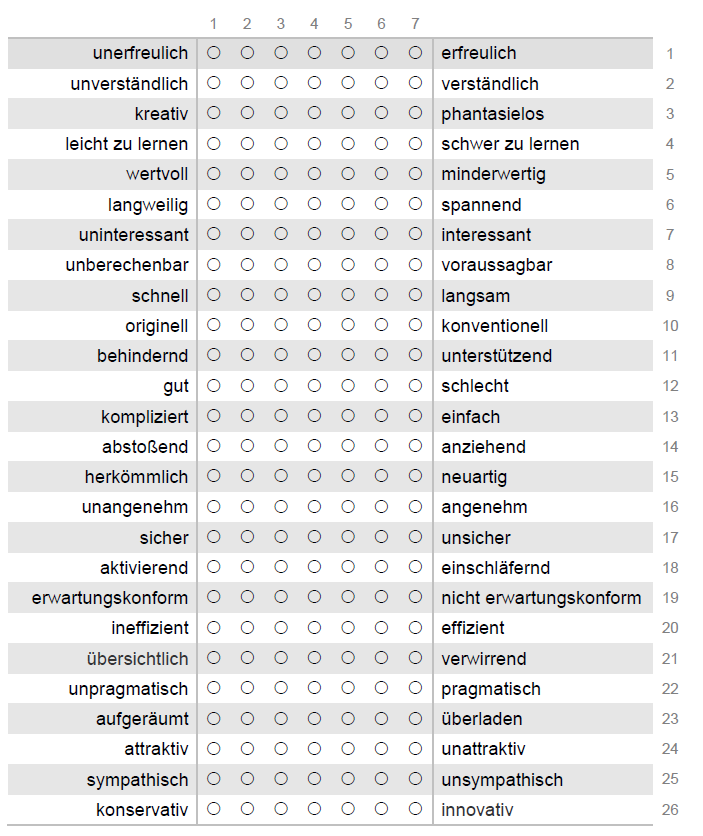
\includegraphics[width=270pt]{res/ueq.png}
\caption{UEQ Fragebogen zur Messung von UX. Der UEQ Fragebogen ist in Form einer Skala mit Gegensatzpaaren von Begriffen gehalten. Die Meinung des Benutzers wird durch das Nähern einem der Gegensatzbegriffe Approximiert.}
\label{ueq}
\end{figure}
\newpage
Diagramme der Studienergebnisse:
\begin{figure}[!ht]
    \centering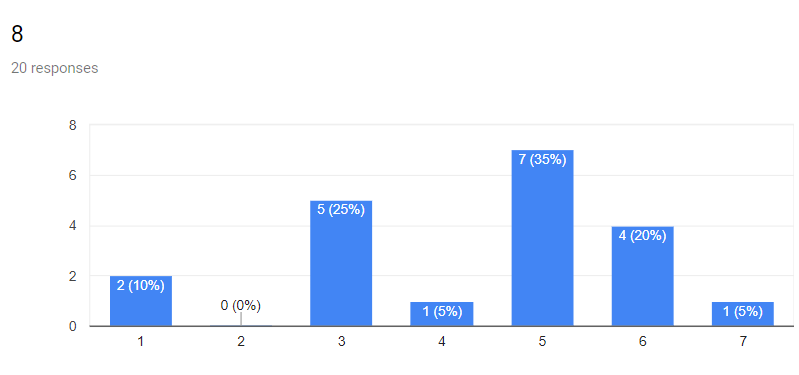
\includegraphics[width=340pt]{res/8_ueq}
\caption{Die Meinungen von Probanden zu der Frage: ''Ist das Programm eher unberechenbar oder voraussagbar''. Die Probanden waren sich bei den Antworten nicht einig.}
\label{item_8}
\end{figure}

\begin{figure}[!ht]
    \centering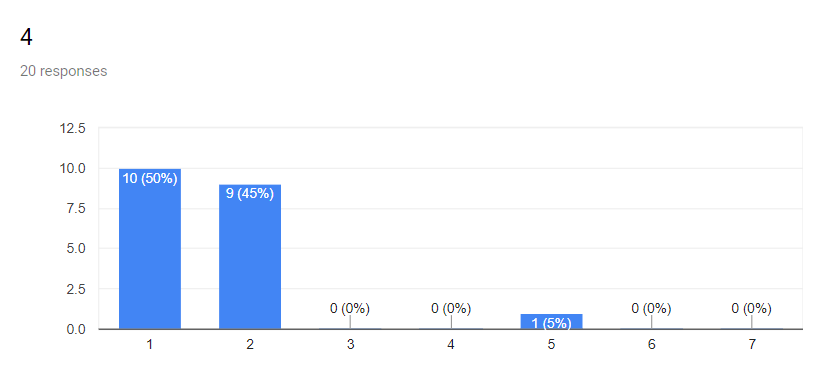
\includegraphics[width=330pt]{res/4_ueq}
\caption{Die Meinungen von Probanden zu der Frage: ''Ist das Programm eher leicht zu lernen oder schwer zu lernen''. 95\% der Probanden haben die Software als sehr leicht oder leicht zu lernen geschätzt.}
\label{item_4}
\end{figure}

\begin{figure}[!ht]
    \centering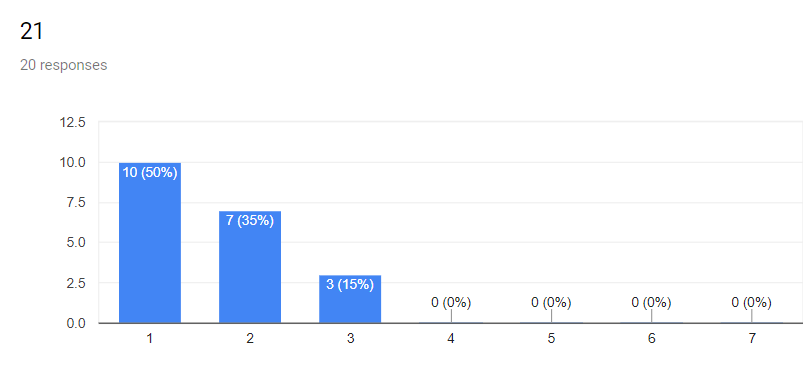
\includegraphics[width=330pt]{res/21_ueq}
\caption{Die Meinungen von Probanden zu der Frage: ''Ist das Programm eher übersichtlich oder verwirrend''. 85\% der Probanden haben die Software als sehr übersichtlich oder übersichtlich geschätzt. 15\% der Probanden fanden die Software relativ übersichtlich.}
\label{item_21}
\end{figure}

\newpage
\subsection{Die UX und Usability Studie}
\paragraph{Einführung für Probanden.}Folgendes Minispiel "Mimicry" ist eine Umsetzung eines IT-gestützten Trainings der sozio-emotionalen Kompetenz. Dieses Training ermöglicht Menschen mit kognitiven Defiziten, zum Beispiel mit einer Autismus Diagnose das Üben der Gesichtsausdrücke. Für manche werden diese Defizite sowohl ein Hindernis in den sozialen Kontakten als auch in dem beruflichen Leben empfunden. Das Training der sozio-emotionalen Kompetenzen erfolgt durch Stärkung der Mimikry Fähigkeit, also der Nachahmung der Emotionen. 
Das Training enthält sowohl die Variante, wo Menschen ihre Ausrücke direkt sehen können als auch die Variante ohne einer Vorschau.
Bitte machen sie sich mit der Einführung vertraut und sobald Sie fertig sind, kann das Spiel angefangen werden.
\label{einf}

\paragraph{Beobachtungen aus der Studienphase}
Während der Studie sind zwei Aspekte besonders aufgefallen, beide bei der Mimikry ohne Vorschau Variante.
Die Probanden waren von der Länge des Anzeigens der Zielemotion gelangweilt. Einige Probanden haben versucht, das Spiel durch anklicken der Hintergrundsfläche zu starten Abb. \ref{knopf}. 
\begin{figure}[!ht]
    \centering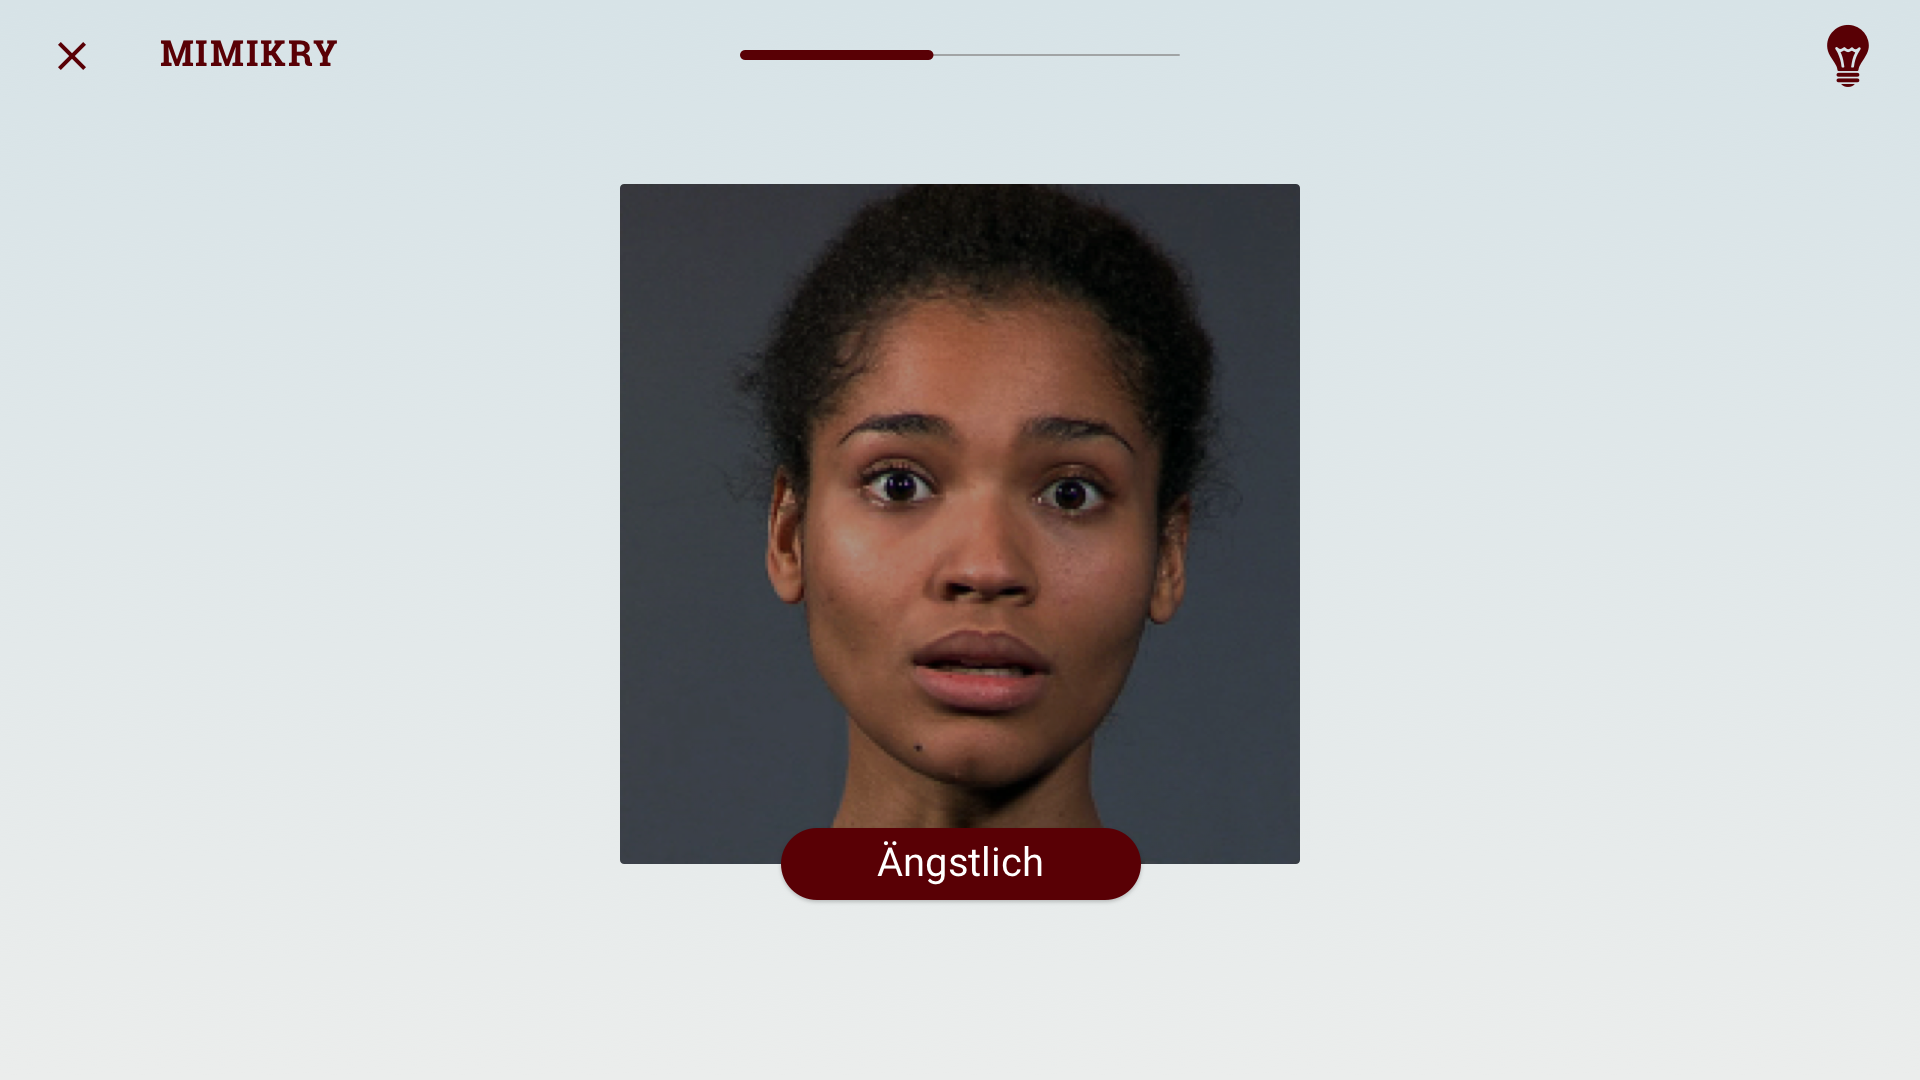
\includegraphics[width=330pt]{res/TASK_MIMIKRY_IIIa.png}
\caption{10 Probanden haben versucht, die Fläche rechts unten anzuklicken, in der Hoffnung, dass das Spiel gestartet wird}
\label{knopf}
\end{figure}
Die Probanden hatten Schwierigkeiten bei der Auffassung des Gesichts von der Kamera. Sie haben nach einem richtigen Winkel gesucht statt die Aufmerksamkeit auf dem Spiel zu fokussieren. 
\begin{figure}
    \centering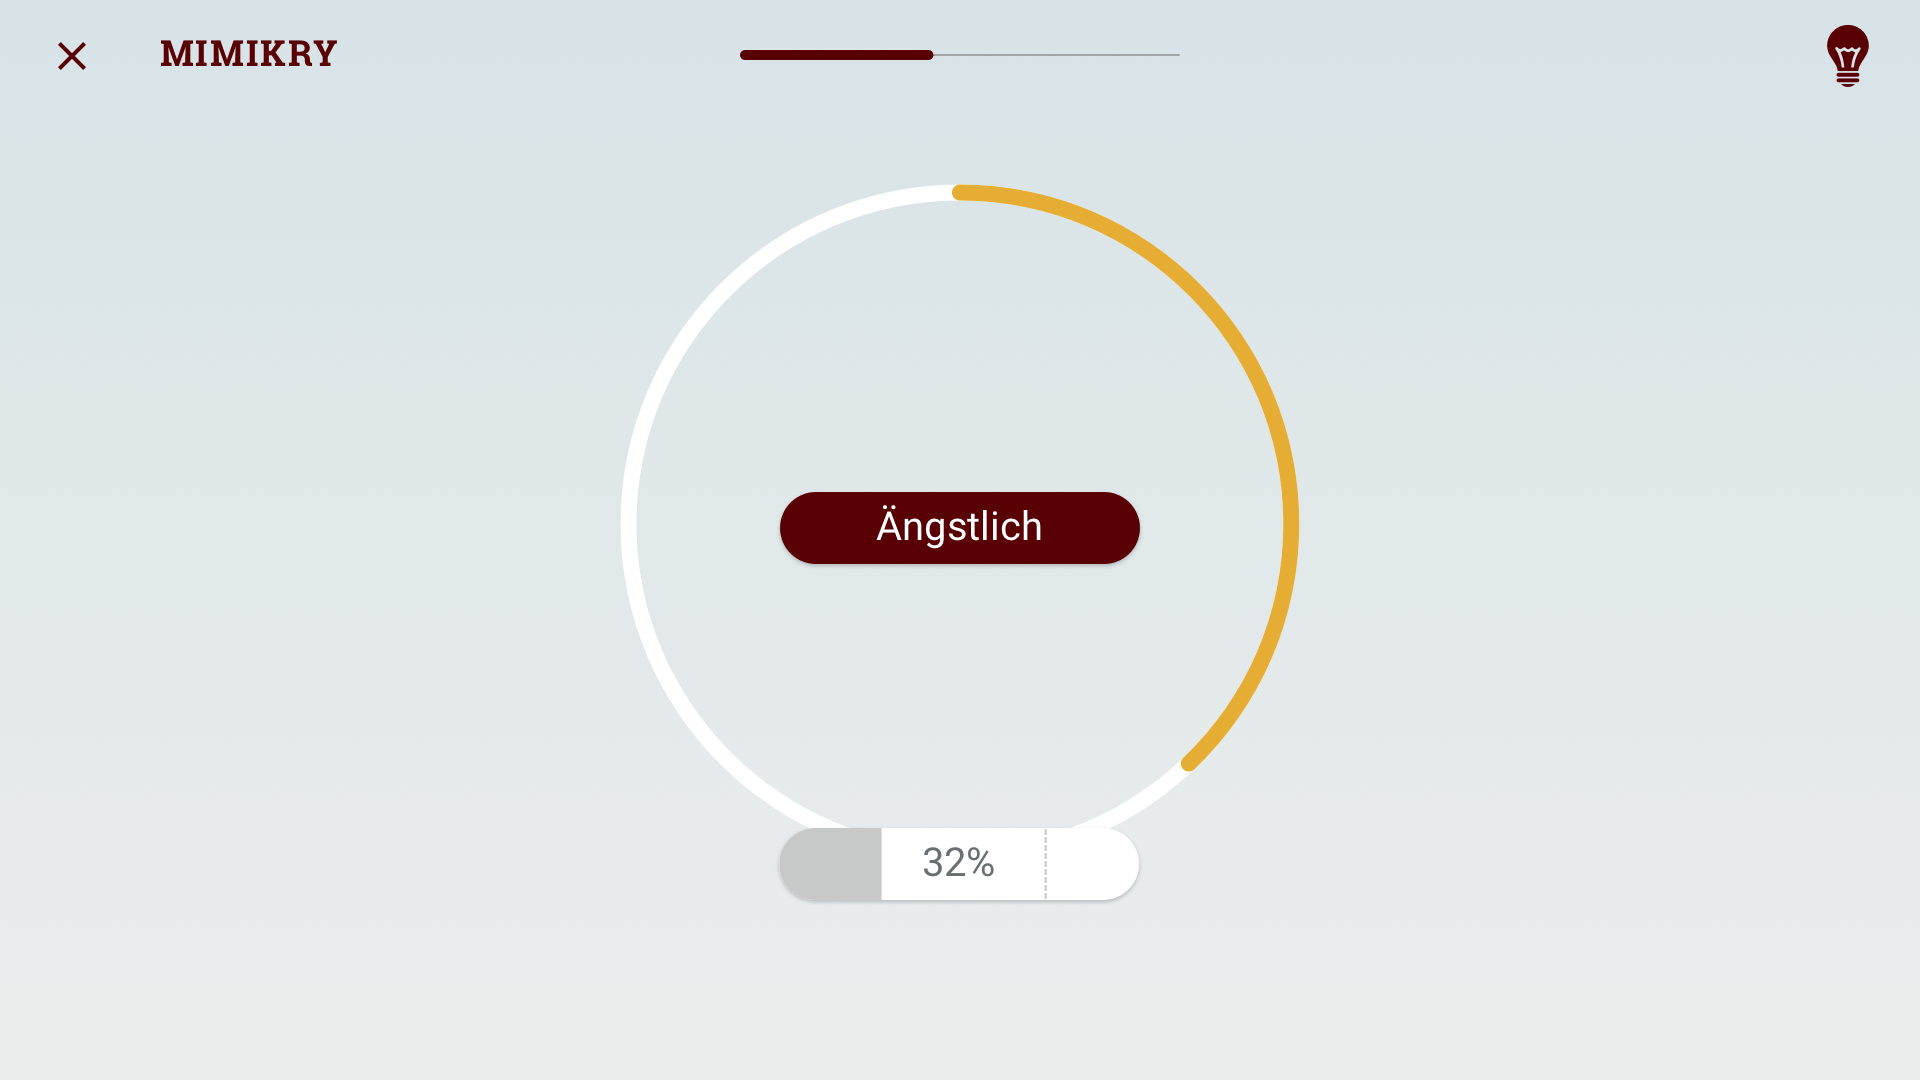
\includegraphics[width=330pt]{res/TASK_MIMIKRY_IIIb.png}
\caption{Fast alle Probanden hatten Schwierigkeiten, den richtigen Winkel der Kamera zu finden, da das Gesicht beim Spielen nicht direkt sichtbar ist. Die Probanden haben durch Lenkung von dem Tablet versucht, die geeignete Kameraposition zu finden. Sie haben darauf geachtet, ob das Gesicht aufgefasst wird, statt sich auf der Aufgabe selbst zu konzentrieren. Die Ursache dafür war manchmal 0\% auf dem Forschrittsbalken, was kein eindeutiges Feedback bezüglich der Qualität der Imitation oder der Auffassung von der Kamera lieferte. }
\label{winkel}
\end{figure}

\paragraph{Bemerkungen der Probanden.}Alle gesammelten Bemerkungen lassen sich zu einer der Kategorien zuordnen. In den Klammern befindet sich die Anzahl der Personen, die diesem Satz ähnliche Bemerkungen getätigt haben:
\begin{enumerate}
    \item Ich bin mir nicht sicher, ob mein Gesicht von der Kamera aufgenommen wird. Es ist frustrierend/ ich fühle mich dadurch unsicher.(14)
    \item Ich finde die App sehr optisch ansprechend(12)
    \item 15 Sekunden sind zu viel für eine Aufgabe(5)
    \item Wie funktioniert der Fortschirttsbalken - soll ich den Gesichtsausdruck einmalig oder über die gesamte Zeit zeigen?(2)
    \item Ich würde mir Bilder oder sogar Videos mit stärker ausgedrückten Zielemotionen wünschen(1)
    \label{quailtat}
\end{enumerate}

\newpage
\subsection{Allgemeine Konzepte der Programmierung}
\paragraph{Screen.}Der Begriff Screen bezeichnet im Android Kontext eine Zusammensetzung mehrerer graphischer Elemente, die auf einmal auf dem Display zu sehen sind. Eine Android App kann aus einem oder mehreren Screens bestehen. Ein Screen ist eine Aktivität oder ein Fragment mit einem zugehörigen Layout.

\paragraph{Interface.}Interfaces ersetzen Mehrfachvererbung in der Sprache Java. Eine Klasse kann mehrere Interfaces (Schnittstellen) implementieren. Alle Methoden innerhalb dieser Schnittstellen muss aber von der Klasse die das Interface implementiert vollständig programmiert werden

\paragraph{Funktion vs. Methode.}Beide sind Anweisungen für die nächsten Schritte, Funktionen erledigen die Aufgaben und geben manchmal einen Wert zurück und Methoden werden nach der Abarbeitung der Aufgaben beendet, ohne jenigen Rückgabewert zu liefern. 

\paragraph{NullPointerException}ist eine in der Java Welt bekannte Fehlermeldung die auftritt, wenn ein referenziertes Objekt nicht existiert, es wurde ihm der Wert null zugewiesen. Bei Mimicry gab es das Gefahr, dass der Presenter mit dem View (siehe Kapitel Implementierung) kommuniziert, wo ein View nicht vorhanden sein könnte. Daher wurden die Schritte unternommen um den Fehler zu vermeiden.

\paragraph{Thread}ist ein Ausführungsstrang oder eine Ausführungsreihenfolge in der Abarbeitung eines Programms. Ein Thread ist Teil eines Prozesses.

\newpage
\subsection{Modul Facepuzzle aus der E.V.A. App}
\begin{figure}[!ht]
    \centering
    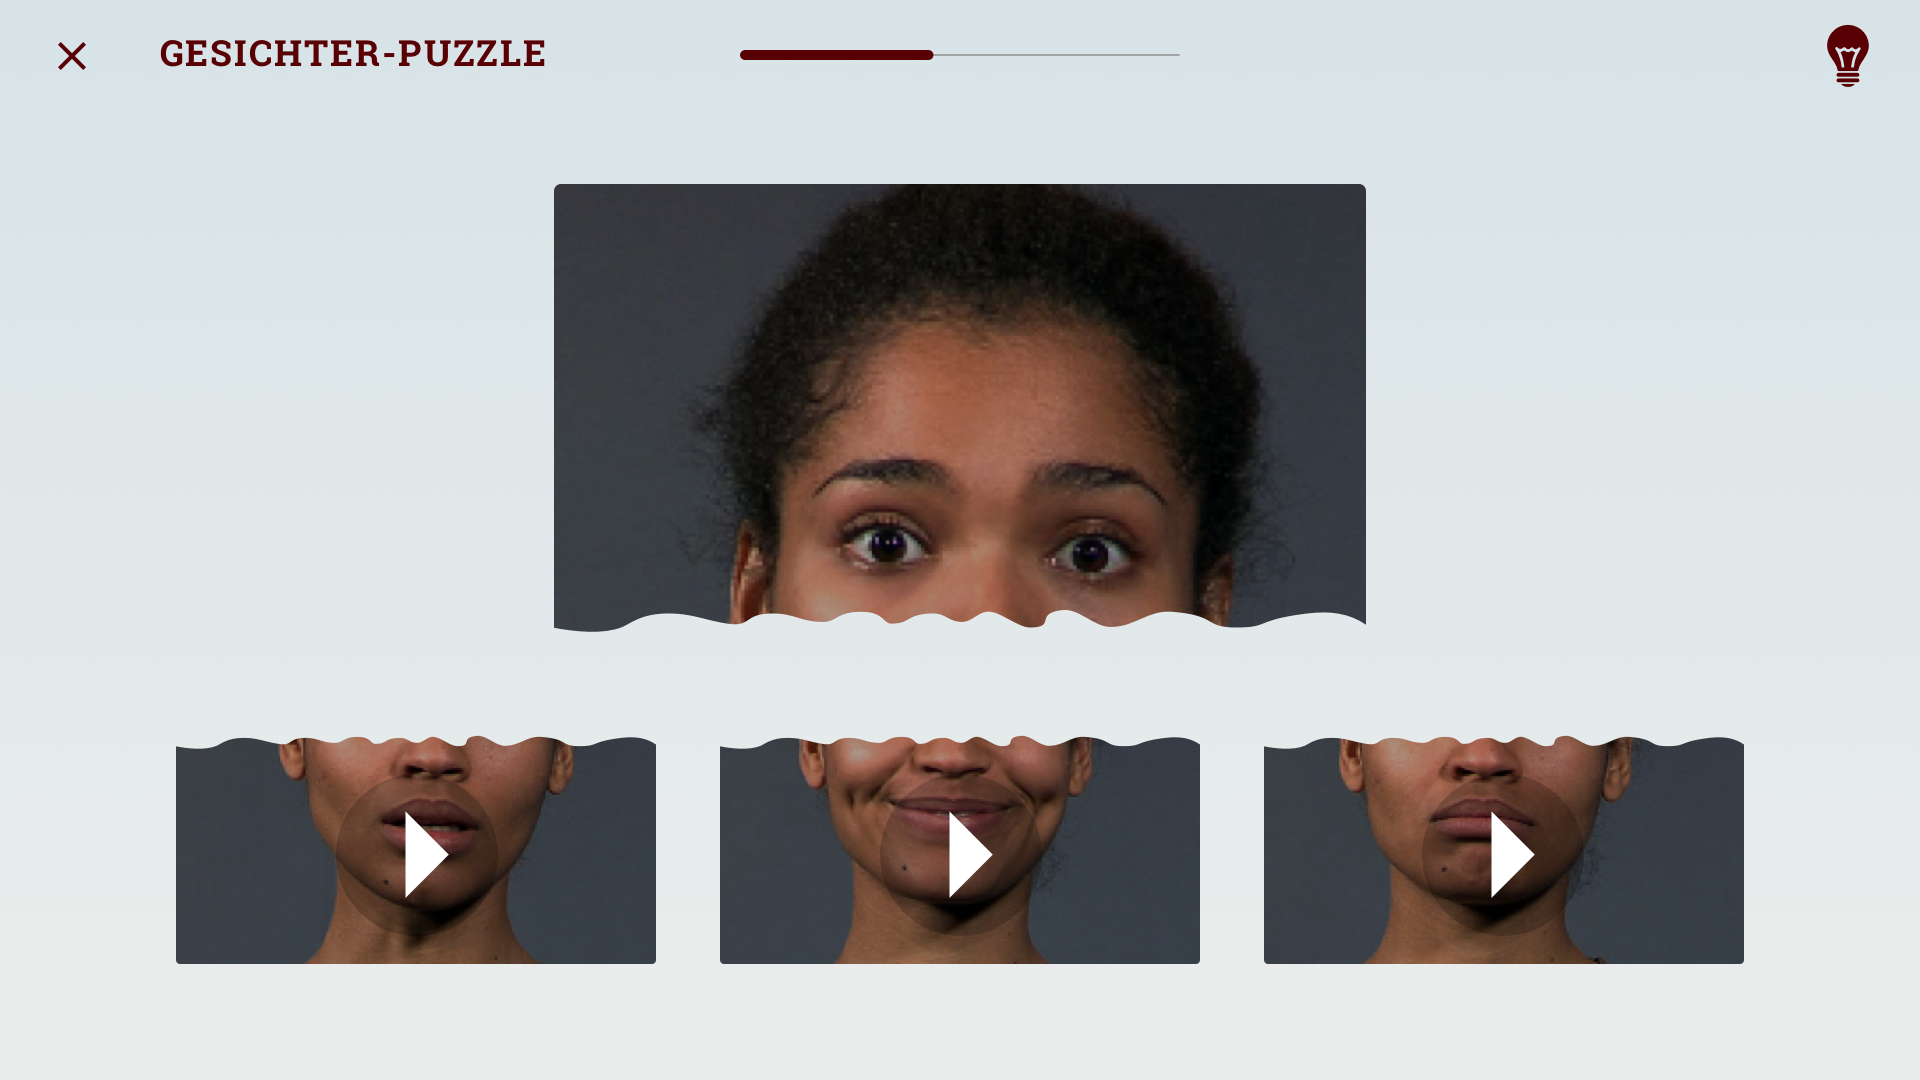
\includegraphics[width=330pt]{res/facepuzzle_implicite.png}
\caption{Gesichterpuzzle implizit: Die Targetemotion wird nur zur Hälfte sichtbar. Drei Videoaufnahmen mit unterer Hälfte des Gesichts der gleichen Schauspielerin werden angezeigt. Sie stellen die Zielemotion und zwei Distraktoren dar. Die Aufgabe ist passende Gesichterteile zu erkennen.}
\label{facepuzzle_implicite}
\end{figure}

\begin{figure}[!ht]
    \centering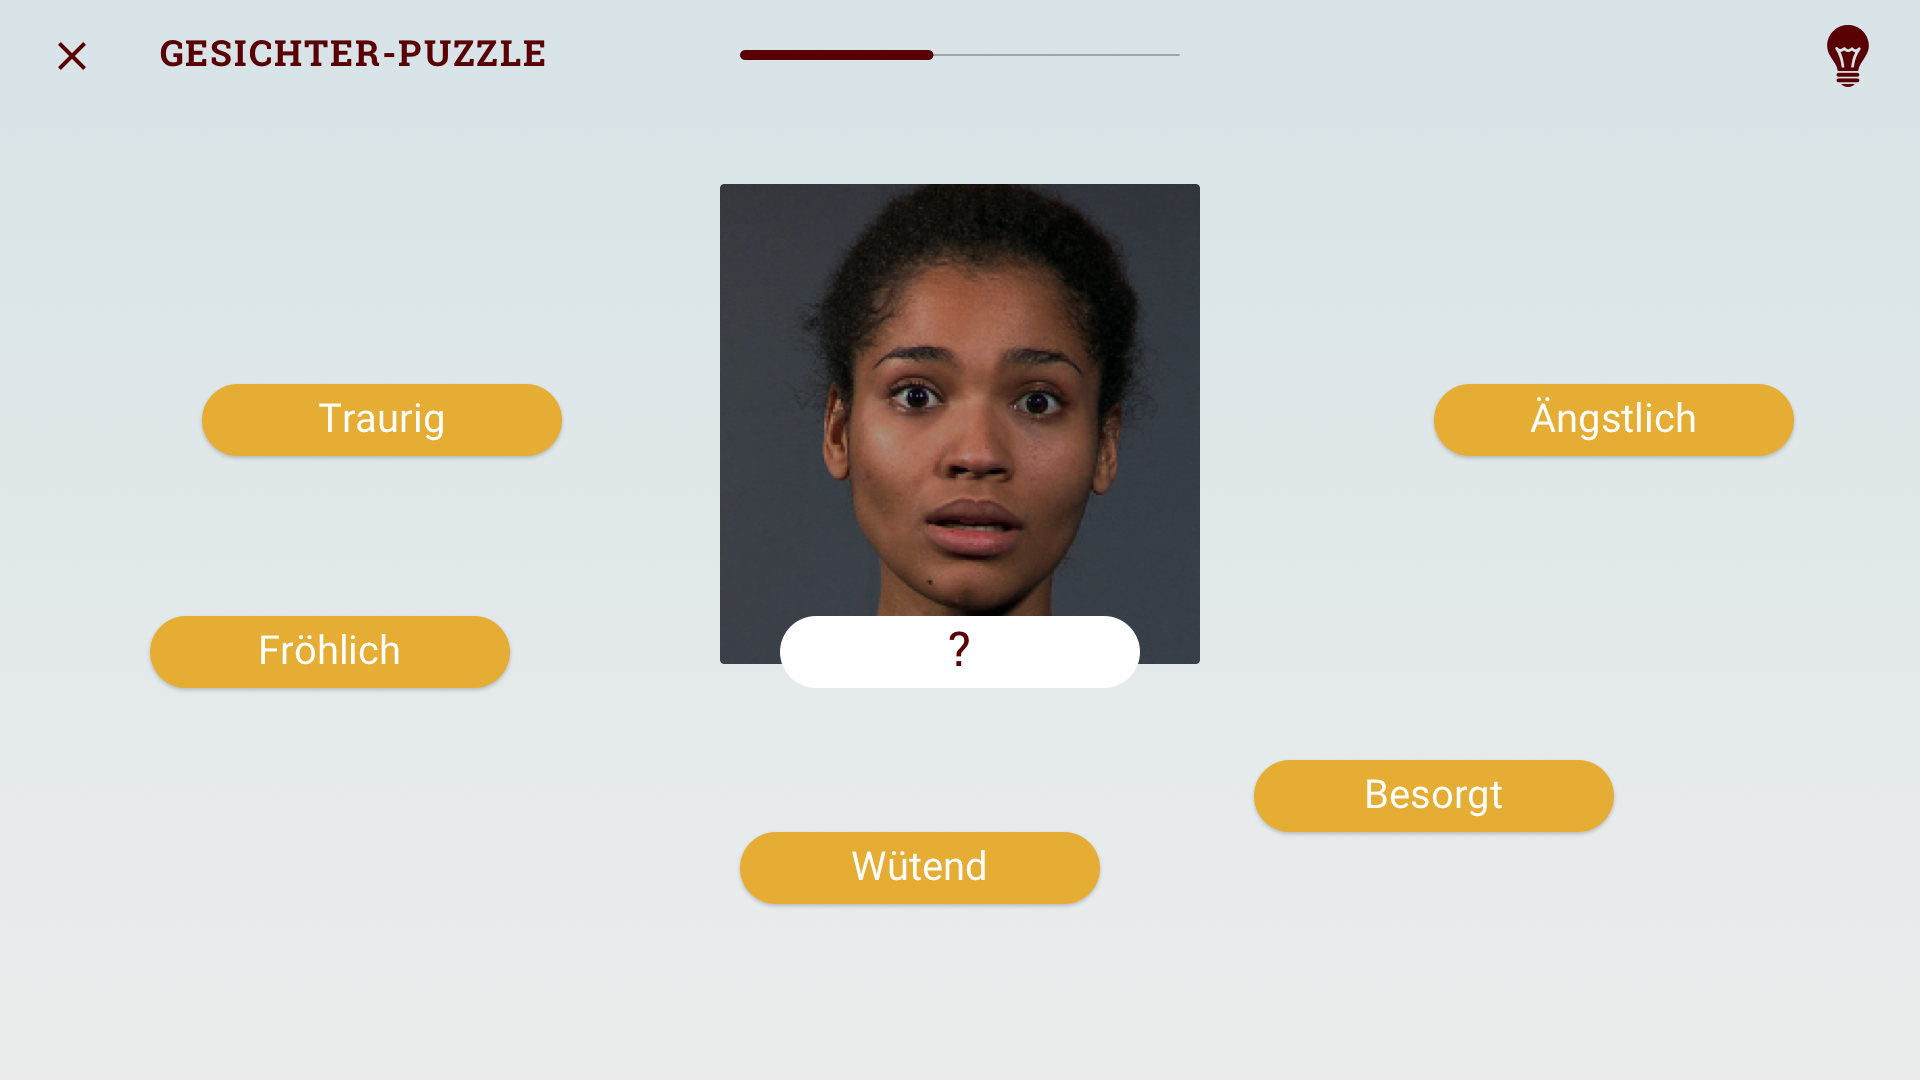
\includegraphics[width=330pt]{res/facepuzzle_explicite.PNG}
\caption{Gesichterpuzzle explizit: Die Targetemotion wird vollständig sichtbar. Mehrere Emotionsnamen werden angezeigt. Die Aufgabe ist die Zielemotion zu identifizieren.}
\label{facepuzzle_explicite}
\end{figure}
